%\begin{figure}[H]
%	\centering
%	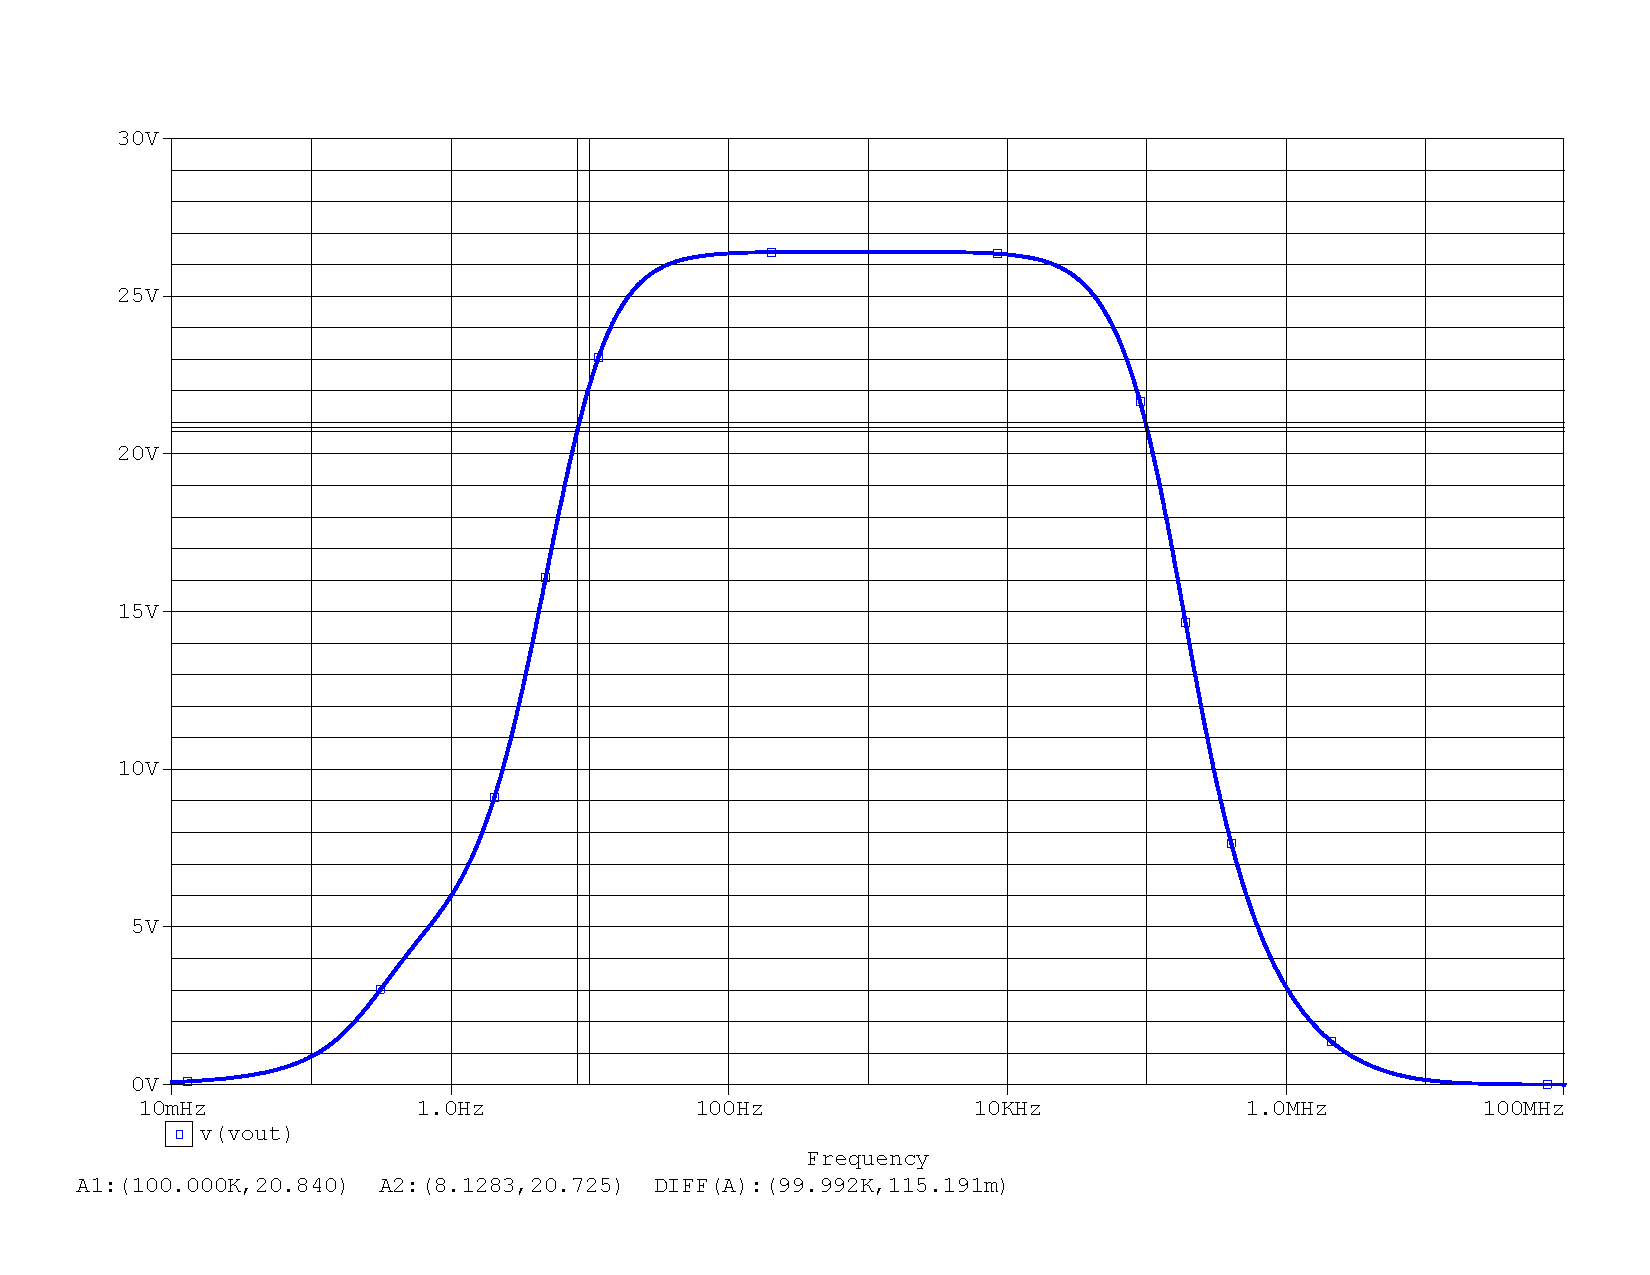
\includegraphics[scale=0.5]{sim_bw_potencia.pdf}
%	\caption{Ancho de banda de potencia}
%	\label{fig:sim_bw}
%\end{figure}

\HgraficarPNG{0.5}{sim_rta_max_potencia.png}{Ancho de banda de potencia}{fig:sim_bw}

El ancho de banda de potencia indica la máxima frecuencia para la cuál el amplificador logra reproducir una señal sinusoidal a máxima potencia. Para este caso, la máxima tensión sin distorsión apreciable es aproximadamente \SI{26}{\volt}. A partir de la figura \ref{fig:sim_bw} se obtiene

\begin{align}
	\centering
	f_L &= \SI{14}{\hertz} \\
	f_H &= \SI{160}{\kilo\hertz}
\end{align}
